% The entire content of this work (including the source code
% for TeX files and the generated PDF documents) by 
% Hongxiang Chen (nicknamed we.taper, or just Taper) is
% licensed under a 
% Creative Commons Attribution-NonCommercial-ShareAlike 4.0 
% International License (Link to the complete license text:
% http://creativecommons.org/licenses/by-nc-sa/4.0/).
\documentclass{article}
\usepackage{fullpage}
% My own physics package
% The following line load the package xparse with additional option to
% prevent the annoying warnings, which are caused by the package
% "physics" loaded in package "physicist-taper".
\usepackage[log-declarations=false]{xparse}
\usepackage{physicist-taper}
\makenomenclature % For an index of symbols.

\title{Continuous Variable Quantum Neural Networks}
\date{\today}
\author{Hongxiang}


\begin{document}


\maketitle
\abstract{
  Notes of arXiv:1806.06871v1
}
\tableofcontents

\section{General continuous variable quantum computation}

Continuous variable quantum computation operates on another model of quantum
computation. A \textit{qumode} is their basic unit of computation. The state of
a qumode could be represented in two different ways:
\begin{enumerate}
  \item A Fock state, $\ket{n}$, where $n\in \mathbb{N}$. They live in a Hilbert
    space called Fock space of countable infinite dimension. Their amplitudes
    squared are probabilities. $n$ represents a state of $n$ bosons
    \footnote{There seems to be no more degree of freedom when $n$ increases. It
    is not clear what $\ket{n}$ means physically. TODO: check this.}. For
    multiple qumodes, the state is represented as
    $\ket{n_0,n_1,\cdots,n_{i-1}}$.
  \item A phase space coordinate $(x,p)$ where $x$ and $p$ are both real
    numbers. They are expectation values of two conjugate operator $\hat{x}$ and
    $\hat{p}$ satisfy certain commutation relations.\footnote{We can think of
      $x$ and $p$ as position and momentum. But each of them gives a complete
      basis $\int \ketbra{x} = \id = \int \ketbra{p}$, so a pair
      $(\vec{x},\vec{p})$ does not transform as a vector anymore.
    }. Note that all coordinates $(\vec{x},\vec{p})$ does not form a
    basis for the Hilbert space. Therefore their amplitudes $F(x,p)$ are not
    probabilities but quasiprobability distributions. For multiple qumodes, the
    state is represented by two vectors $(\vec{x}, \vec{p})$.
\end{enumerate}

\textbf{Note}: 
\begin{enumerate}
  \item This infinite-dimensional Fock space cannot be simulated classically.
    What they do is to cut-off the dimension above a number, so that the Hilbert
    space is truncated. This creates unnormalised state in simulation. To
    address this issue, they add a penalty as a regularisation term in their
    cost function as:

    $$
    P(\{\ket{\psi_{x_i}}\}) = 
    \sum_i \left( |\braket{\psi_{x_i} | \Pi_H | \psi_{x_i}}| - 1\right)^2
    $$,

    where $\Pi_H$ projects onto the truncated Hilbert space. It is not clear how
    this penalty term could actually be implemented on their quantum computer.
  \item The phase-space picture is more convenient to represent the
    transformations in continuous-variable quantum computation.
\end{enumerate}

\subsection{ General transformation on CV model and embedding classical neural
network}

Written in the phase-space picture, the transformations on CV-quantum
computation can be divided into Gaussian or non-Gaussian gates.

\textbf{ Gaussian}:
The Gaussian gates in general transform a ket $\ket{\vec{x},\vec{p}}$ according
to the following rule:

$$ 
\begin{pmatrix}
  \vec{x} \\ \vec{p}
\end{pmatrix}
\to 
M \begin{pmatrix}
  \vec{x} \\ \vec{p}
\end{pmatrix}
+ 
\begin{pmatrix}
  \vec{\alpha_r}\\ \vec{\alpha_i}
\end{pmatrix}
$$

Here $M$ is a sympletic real matrix of size $2N\times 2N$, $\vec{\alpha_r}$
and $\vec{\alpha_i}$ are real and complex part of a complex vector
$\vec{\alpha}\in \mathbb{C}^{N}$. 

Importantly, $M$ is of size $2N\times 2N$ and has a lot of freedom inside (i.e.
its submatrix could be non-sympletic). \textbf{When we only use the $\vec{x}$ to
do quantum computation} (i.e. we care only about $\vec{x}$ and avoid computations
that mixes $\vec{x}$ and $\vec{p}$), arbitrary real matrix $W$ of size $N\times
N$ could be implemented using Gaussian gates. Together with the affine
transformation, this means any linear neural network of weight $W$ and bias
$\vec{b}$ could be implemented using quantum computations such that (discussed
in page 6):

$$
D\circ U_2 \circ S \circ U_1 \ket{\vec{x}} = \ket{W\vec{x} + \vec{b}}
$$


\textbf{Non-Gaussian}: The non-Guassian gates achieves a nonlinear function
\footnote{It is not clear to me what kind of non-linear function could be
achieved, TODO check.} on the phase space vector $\vec{x}$:

$$
\Phi \ket{\vec{x}} = \ket{\phi(\vec{x})}
$$

Specifically, the gate $V = \exp(-i \phi(\hat{x}_i)\otimes \hat{p}_{i'})$ maps
$\ket{x}\ket{0} \to \ket{x}\ket{x+\phi(x)}$. With a swap gate, they could
achieve $\ket{x_i} \to \ket{\phi(x_i)}$. Here $\phi(x)$ is a polynomial of a
fixed degree\footnote{Why use a polynomial function $\phi$? Why not just use any
function you want?}, so any smooth function could be approximated by their
Taylor expansion. Sadly, they do not have a decomposition of $V$ in terms of
elementary CV quantum gates.

Together with the Gaussian gates, they have the embedding of an arbitrary
classical neural network of the form $\Phi(W\vec{x}+\vec{b})$ as a quantum
neural networks in their Fig.1. Note that in practice, they use the Kerr gate
$K(\kappa) = \exp(i\kappa \hat{n}^2)$ as a their nonlinear function.

\subsection{Note about non-linearity}
\label{sec:Note about non-linearity}

Quantum mechanics is linear, but only in terms of different kets/vectors. Since
circuit model quantum allows any (nonlinear) function on binary number
$f(b_1,\cdots,b_n)$ to be represented by a quantum gate
$U:\ket{b_1,\cdots,b_n}\to \ket{f(b-1,\cdots,b_n)}$, their proposal is not very
exciting in bring nonlinearity.\footnote{Thank Andrea for pointing this out.}
However, their model is exciting in that:
\begin{enumerate}
  \item Their model naturally acts on real numbers $x$ without the need to
    encode them into binary strings.
  \item They divide between linear (Gaussian gate) and nonlinear (non-Gaussian
    gate) in their quantum neural layer is quite clear and quite resembles the
    structure of conventional neural network. In out circuit model quantum
    computation, I have not ever seem something like this.
\end{enumerate}

I think we have:

\begin{table}[H]
  \centering
  \caption{Non-liearity}
  \begin{tabu}{X[0.5] X X}
    Input & Encoded as & Linear? \\
    \hline
    Classical data & Angles of gates & No, usually the quantum gate are
    nonlinear w.r.t their parameters \\
    \hline
    Classical data & Encoded in the amplitudes of
    $\sum_{b_1,\cdots,b_n}x_{b_1,\cdots,b_n}\ket{b_1,\cdots,b_n}$ & 
    In circuit model, this depends on the data encoding layer. But any
    transformation after are linear except from measurements. 
    \\
    % -----
    & Encoded in basis of either $(\vec{x},\vec{p})$ or $\ket{b_1,\cdots,b_n}$ & 
    The transformation on them could be nonlinear.
    \\
    \hline
    Quantum data & Encoded as probability amplitudes & Linear except from
    measurements. \\
    % ------
    & Encoded as quasiprobability amplitudes (in CV model) & ???\footnote{Todo:
  check this.}
  \end{tabu}
\end{table}

The general transformation on $N$ qumodes are devided into two categories: the Gaussian gates and non-Gaussian gates. 

\section{ CV-QNN models and experiments}

\subsection{Models}

The paper also discusses how many specific neural network structure could be  implemented as in a quantum neural network. This includes: 

\begin{itemize}
  \item \textbf{Convnet}: implemented just as a special matrix (of Toeplitz
    structure) to do the convolution. They have detailed how this matrix could
    be achieved in terms of the Gaussian matrix $M$ but not decomposition
    in terms of the elementary CV quantum gates ($R,D,S,BS$) is provided.
  \item \textbf{RNN}: implemented by reusing the same parameter for the quantum
    layer. Also, it is very convenient to connect the output of a CV quantum
    computer back to its input on a optical implementation of CV quantum
    computer
  \item \textbf{Residual Network}: implemented using the $V$ gate previously
    mentioned, which maps $\ket{\vec{x}}\ket{0}~\to~\ket{x}\ket{\vec{x} + \phi(\vec{x})}$.
\end{itemize}

\subsection{Training algorithm}

They have a very short simple discussion of the training algorithm. They use
their framework in TensorFlow to do the training and so they can either use the
build-in automatic differentiation, or numerical difference to do this training.
Adam seems to be the best choice, but they have not reported the hyperparameters.
\begin{figure}[H]
  \centering
  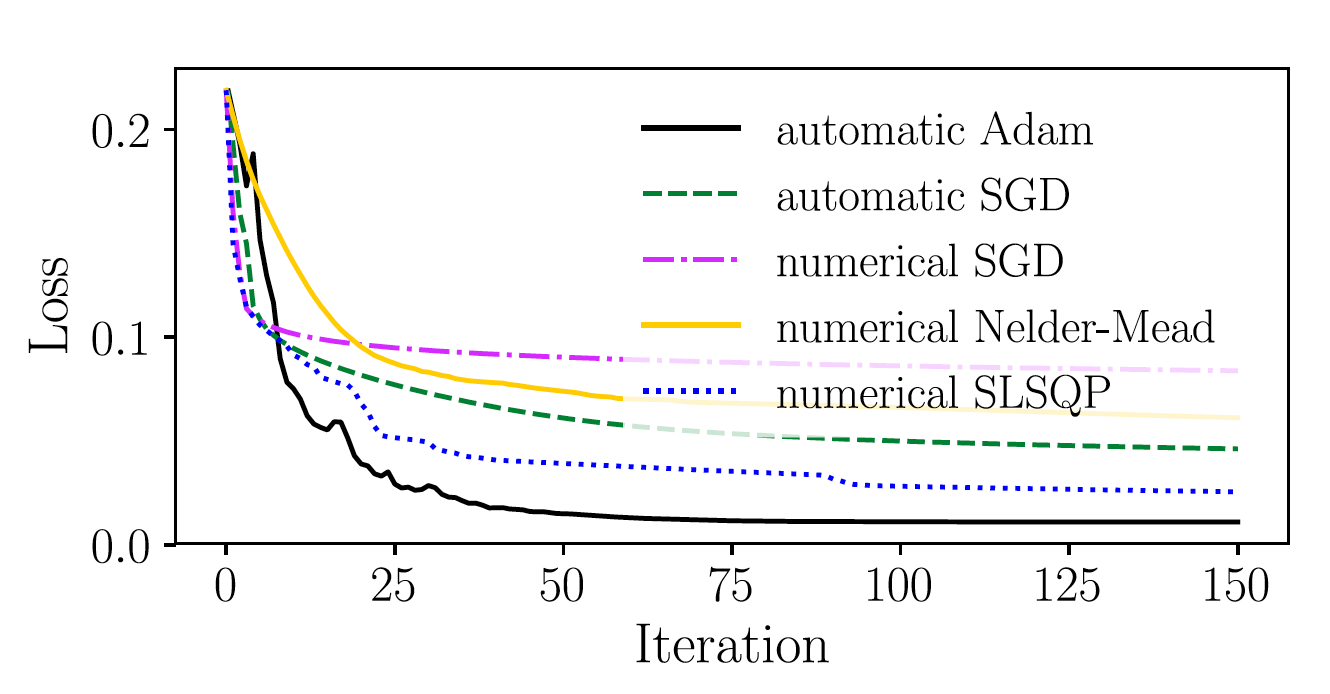
\includegraphics[width=0.8\linewidth]{opt.png}
  \caption{Optimiser}
\end{figure}

\subsection{ CV-QNN Experiments}

\begin{table}[H]
  \centering
  \extrarowsep=1.5mm
  \begin{tabu}{X[0.5]|X|X|X|X}
    & Function fitting & Classifying data & Generating image & Auto-encoder 
    \\
    Purpose &
    Produce a circuit which fits the function
    $\ket{x} \overset{\text{circuit}}{\to} \ket{f(x)}$.&
    Classify whether the transaction is genuine or fraud. &
    For $m$ size $N\times N$ matrices, choose $m$ initial state $\ket{\phi_\alpha}$
    ($\alpha = 1,\cdots m$), find a circuit that transform $\ket{\phi_\alpha}$
    into a specific quantum encoding of matrix $\ket{A_\alpha}$ for each
    image. &
    Find a circuit which encodes all states with at most two phonons
    $\ket{\phi}=\alpha\ket{0} + \beta\ket{1} +\gamma\ket{2}$ into a phase space
    coordinate $(x,p)$.
    \\
    Circuit &
    \includegraphics[width=1.00\linewidth]{A.pdf} &
    \includegraphics[width=1.00\linewidth]{B.pdf} &
    \includegraphics[width=1.00\linewidth]{C.pdf} &
    \includegraphics[width=1.00\linewidth]{D.pdf} 
    \\
    Input &
    $x \overset{\mathcal{D}}{\to} \ket{(\vec{x},0)}$, data encoded as
    phase space coordinate.&
    Data are processed after a classical layer, and then encoded as angles of circuit.&
    Data are quantum states $\ket{\phi_\alpha}$, each one $\alpha$ is supposed
    to generate a distinct image.&
    Before training, the data are processed by classical layer and then input
    into the quantum layer as phase space coordinate. After training, the encoder accepts two angles as
    the input.
    \\
    Output &
    Output a measured value, which is a real number, interpreted as the function evaluated at $x$. &
    Output a measured value, which is the number of photons in each mode. By
    post-selecting on single-photon outputs, the position of this photon will be
    interpreted as the decision.&
    Output a quantum state, which should be as closed as possible to the state:
    $\ket{A_\alpha} \propto \sum_{i,j} \sqrt{a_{ij}^\alpha} \ket{i,j} $. Here
    $\alpha$ labels the different matrices. $a_{ij}^\alpha$ is the corresponding
    matrix element.
    &
    Output the state 

    $\ket{\psi} = \alpha\ket{0} + \beta\ket{1} +
    \gamma\ket{2}$.
    \\
    Cost function &
    $\sum_i \left[f(x_i) - \braket{\hat{x}} \right]^2$ plus
    regularisation terms. Here $\braket{\hat{x}}$ is the expectation value after
    the quantum circuit.&
    $\sum_{i\in \text{data}} (1-p_i)^2$, $p_i$ is the probability of correct
    detection.&
    $\sum_i |\braket{\psi_i | A_i}|^2$ plus regularisation terms. 
    Requires a CV version of C-SWAP test to get $|\braket{\psi_i |
    A_i}|$ (not mentioned in the paper).
    &
    $\sum_i \left(|\braket{ i| \psi_i }|^2 -1\right)^2$ plus regularisation terms.
    Requires a CV version of C-SWAP test to get $|\braket{\psi_i |
    A_i}|$ (not mentioned in the paper).
    \\
    Result (figure in the paper) &
    Fig.5 & Fig.9 & Fig.10 & Fig.11 
  \end{tabu}
\end{table}

\section{License}
The entire content of this work (including the source code
for TeX files and the generated PDF documents) by 
Hongxiang Chen (nicknamed we.taper, or just Taper) is
licensed under a 
\href{http://creativecommons.org/licenses/by-nc-sa/4.0/}{Creative 
Commons Attribution-NonCommercial-ShareAlike 4.0 International 
License}. Permissions beyond the scope of this 
license may be available at 
\href{http://www.google.com/recaptcha/mailhide/d?k=015LguzBJigi0rpyuJRqLoig==\&c=p1c-M-mm7ZcjUCkTuZZa9eEPHRVk6paN0694iazlQy8=}
{[My Email Address(Click)]}.

\bibliography{cite}{}
\bibliographystyle{alphaurl}
% \begin{thebibliography}{1}
% 	\bibitem{book} 
% \end{thebibliography}
\printnomenclature

\end{document}
